\subsection{Example}%
\label{subsec:kgraph_example}
An example \ac{kgraph} can be visualized in \Cref{fig:kgraph_example}, where parameterization of edges is displayed, and the object on which that \ac{kgraph} holds information is displayed as an image. For clarification, the connected left part with the image of the point robot on the center node has three outgoing edges that describe robot driving. The connected part on the right with an image of the point robot and the green box on the center node has two outgoing edges that describe the robot pushing against the green box.\bs

\begin{figure}[H]
    \centering
    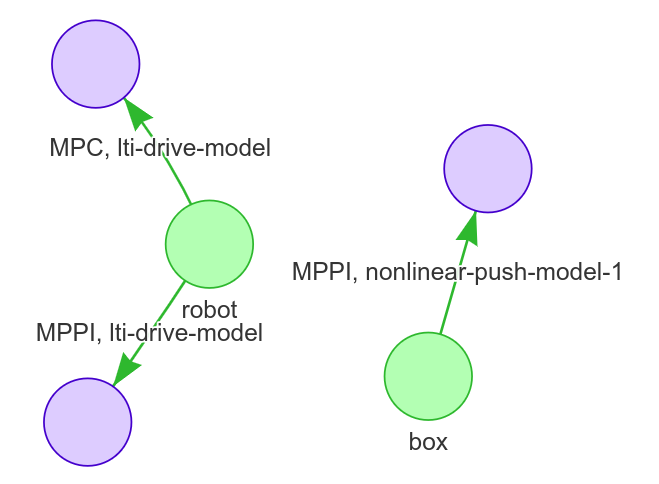
\includegraphics[width=10cm]{figures/proposed_method/kgraph_example}
    \caption{The \ac{kgraph} that collected action feedback on two objects. Three edge parameterizations to drive the robot and two edge parameterizations to push the green box.}%
    \label{fig:kgraph_example}
\end{figure}

The edges in the figure above display only the edge parameterization but store more information, mainly the success factor. The blue nodes serve a small purpose, ensuring edges can point to a node. The blue nodes could fulfill a larger purpose, describing which actuators the edge can control. For example, a mobile robot with a robot arm attached can have a set of controllers that only drive the base, a set of controllers that only steer the robot arm and a set that controls both the base and robot arm. In such cases, the blue nodes describe which part of the robot can be actuated. The controllers considered in this thesis control every robot actuator, resulting in the blue nodes serving such a small purpose.\bs
